\chapter{DESARROLLO DEL TRABAJO}

\section{Backup y Restauración}
\subsection{RMAN}
El Recovery Manager (RMAN) es una utilidad usada para respaldar (backup), restaurar, recuperar y clonar bases de datos ORACLE.

Este producto se encarga de la gestión de backups y restauración de data files, archive logs y control files, además de poder ser usado para la recuperación completa o incompleta de una Base de datos.

Rman tiene la característica de ser configurado de dos formas , la primera, más limitada y con menos opciones , que solo puede gestionar una sola base de datos y donde toda la información de los backups es guardada en el controlfile y la segunda, más completa y robusta, manejado por un repositorio que se guarda en la base de datos en forma de esquema y que nos permitirá la gestión de backups de un mayor número de instancias.

RMAN puede ser operado desde Oracle Enterprise Manager o desde linea de comandos.La mayor ventaja de RMAN es que sólo se utiliza el espacio de copia de seguridad en la base de datos.

RMAN nos permite realizar backup ya sea en frío o en caliente.

Ejemplo de RMAN:

\begin{list}{}{}
\item [oracle@localhost oracle] \$ rman
\item Recovery Manager: Release 10.1.0.2.0 - Production Copyright (c) 1995, 2004, Oracle. All rights reserved.
\item RMAN> connect target;
\item connected to target database: ORCL (DBID=1058957020)
\item RMAN> backup database;
\end{list}


\subsection{Backups de la BD en Frio}
Los backups en frio implican parar la Base de Datos en modo normal y copiar todos los ficheros sobre los que se asienta(datafile,controlfile y logfile). Antes de parar la Base de Datos hay que parar también todos las aplicaciones que estén trabajando con la Base de Datos. Una vez realizada la copia de los ficheros, la Base de Datos se puede volver a arrancar.

Los pasos que hay que seguir para realizar un backup en frió(en oracle) serían:

\begin{enumerate}
\item Conocer y listar la ubicación de los datafiles, controlfiles y logfiles. Esto se hace ejecutando:
\begin{itemize}
\item select file\_name from dba\_data\_files; 
\item select name from v\$controlfile;
\item select member from v\$logfile;
\end{itemize}
\item Detener la base de datos mediante shutdown normal o inmediato.
\item Copiar los archivos datafiles, controlfiles y logfiles a un medio de backup preferido como cinta, disco duro, otra máquina, etc.
\end{enumerate}

\textbf{Ventajas:}
\begin{itemize}
\item Fácil de ejecutar y automatizar.
\item El tiempo de recuperación es predecible. Solo hay que conocer el tiempo de transferencia de los ficheros donde reside el backup.
\end{itemize}

\textbf{Desventajas:}
\begin{itemize}
\item No es posible utilizar la base de datos mientras el backup se este realizando.
\item La recuperación de la base de datos es siempre completa.
\end{itemize}

\textbf{Cuando debe Usarse?}

Cuando lo que se necesita es tener una copia de la base de datos completa y que no
sera recuperada con frecuencia.


\section{Backups de la BD en Caliente}
El backup en caliente se realiza mientras la Base de Datos está abierta y funcionando en modo ARCHIVELOG. Habrá que tener cuidado de realizarlo cuando la carga de la Base de Datos sea pequeña.

Este tipo de backup consiste en copiar todos los ficheros correspondientes a un tablespace determinado, los ficheros redo log archivados y los ficheros de control. Esto para cada tablespace de la Base de Datos.

El backup en caliente consiste en 3 procesos:

\begin{enumerate}
\item Copiar los datos del tablespace.
\item Copiar los redo logs archivados.
\item Copiar los control file.
\end{enumerate}

\textbf{Ventajas:}
\begin{itemize}
\item La base de Datos se puede utilizar mientras se realiza el backup.
\item Se puede realizar incluso con usuarios accesando la Base de Datos.
\end{itemize}

\textbf{Desventajas:}
\begin{itemize}
\item Ocupa mucho mas tiempo que el de un backup en frio.
\item La Base de Datos debe estar operando en modo ARCHIVELOG.
\item Sólo se debe hacer durante los períodos de bajo uso.
\end{itemize}

\textbf{Cuando debe Usarse?}

Cuando la implantación de Base de Datos requiere disponibilidad de la misma 24h. al
día, 7 dias a la semana.

\section{Estado del Arte}
Se entiende por Información al conjunto de datos que han sido procesados con la finalidad de establecer un mensaje y generar conocimiento del sistema que lo reciba. El dato es su unidad mínima, el cual por sí solo no posee ningún valor, pero en conjunto genera información. Esta información al ser organizada adecuadamente se convierte en conocimiento y luego del resultado de su análisis se convierte en finalmente sabiduría. \citeA{Blanco2013}

\subsection{Estrategias de Respaldo}

\begin{equation}
f(x)= \left\{ \begin{array}{l||c|l}
x^2 & \mbox{ si } & x<0 \\ \hline
& & \\
x-1 & \mbox{ si } & x>0
\end{array}
\right.	
\end{equation}

\begin{table}[ht]
\centering{
    \fontfamily{ptm}
        \selectfont{
            \rowcolors{1}{gray}{cyan}
            \begin{tabular}{ll}
                $x_{n+1}$ & $|x_{n+1}-x_n|$\\ \hline
                1.20499955540054 & 0.295000445\\
                1.17678931926590 & 0.028210236\\
                1.17650196994274 & 0.000287349\\
                1.17650193990183 & 3.004$\times10^{-8}$\\
                1.17650193990183 & 4.440$\times10^{-16}$\\ \hline
            \end{tabular}
}}
\caption{Iteracion de Newton para $x^2-\cos(x)-1=0$ con $x_0=1.5$}
\end{table}


Este un ejemplo de imagen

\begin{figure}[ht]
\centering
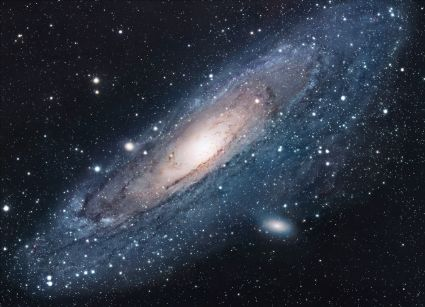
\includegraphics[scale=1.7]{images/universe.jpg}
\caption{The Universe}
\label{fig:universe}
\end{figure}

Terminamos

\subsection{Estrategias de Recuperaci\'on}

\begin{table}[ht]
\centering{
    \fontfamily{ptm}
        \selectfont{
            %\rowcolors{1}{gray}{cyan}
            \begin{tabular}{ll}
                Actividad & Duraci\'on\\ \hline
                Elaboración de los Aspectos Generales del Trabajo de Investigaci\'on   &   10 d\'ias\\
                Elaboración del Marco Te\'orico   &   35 d\'ias\\
                Elaboración del Marco Metodol\'ogico   &   15 d\'ias\\
                Elaboración del Marco Metodol\'ogico   &   15 d\'ias\\
                1.17650193990183 & 4.440$\times10^{-16}$\\ \hline
            \end{tabular}
}}
\caption{Cronograma}
\end{table}